% ===================================================================
% main.tex
% Archivo principal de la presentación Beamer
% Análisis Predictivo de Churn en Telecomunicaciones
% ===================================================================

\documentclass[11pt, aspectratio=169]{beamer}

% ===================================================================
% PREÁMBULO: Configuraciones y paquetes
% ===================================================================
% ===================================================================
% preamble.tex
% Configuraciones globales, paquetes y comandos personalizados
% ===================================================================

% ===================================================================
% PAQUETES Y CONFIGURACIONES DE IDIOMA
% ===================================================================
\usepackage[utf8]{inputenc}
\usepackage[spanish]{babel}
\usepackage{csquotes}
\usepackage{graphicx}
\usepackage{booktabs}
\usepackage{array}
\usepackage{multirow}
\usepackage{colortbl}
\usepackage{tikz}
\usepackage{amsmath}
\usepackage{amsfonts}
\usepackage{amssymb}
\usepackage{hyperref}
\usepackage{xcolor}
\usepackage{listings}
\usepackage{caption}
\usepackage{subcaption}
\usepackage{siunitx}
\usepackage{pgfplots}
\pgfplotsset{compat=1.17}
\usetikzlibrary{shapes,arrows,positioning,fit,backgrounds}

% ===================================================================
% CONFIGURACIONES DE BEAMER
% ===================================================================
\usetheme{Madrid}
\usecolortheme{default}

% Configuración de colores personalizados
\definecolor{primary}{RGB}{0, 51, 102}      % Azul institucional
\definecolor{secondary}{RGB}{184, 1, 68}    % Rojo corporativo
\definecolor{accent}{RGB}{46, 134, 171}     % Azul acento
\definecolor{success}{RGB}{46, 204, 113}    % Verde éxito
\definecolor{warning}{RGB}{241, 196, 15}    % Amarillo advertencia
\definecolor{danger}{RGB}{231, 76, 60}      % Rojo peligro

% Configuración del tema de colores
\setbeamercolor{title}{fg=white, bg=primary}
\setbeamercolor{frametitle}{fg=white, bg=primary}
\setbeamercolor{structure}{fg=primary}

% Personalización de bloques
\setbeamercolor{block title}{bg=primary, fg=white}
\setbeamercolor{block body}{bg=primary!10}

\setbeamercolor{block title example}{bg=success, fg=white}
\setbeamercolor{block body example}{bg=success!10}

\setbeamercolor{block title alerted}{bg=danger, fg=white}
\setbeamercolor{block body alerted}{bg=danger!10}

% Configuración de la tabla de contenidos
\setbeamertemplate{section in toc}{%
    \hspace{0.5em}%
    \inserttocsectionnumber.~\inserttocsection%
}

% Configuración de los footers
\setbeamertemplate{footline}{%
    \leavevmode%
    \hbox{%
        \begin{beamercolorbox}[wd=.333333\paperwidth,ht=2.25ex,dp=1ex,center]{author in head/foot}%
            \usebeamerfont{author in head/foot}\insertshortauthor
        \end{beamercolorbox}%
        \begin{beamercolorbox}[wd=.333333\paperwidth,ht=2.25ex,dp=1ex,center]{title in head/foot}%
            \usebeamerfont{title in head/foot}\insertshorttitle
        \end{beamercolorbox}%
        \begin{beamercolorbox}[wd=.333333\paperwidth,ht=2.25ex,dp=1ex,right]{date in head/foot}%
            \usebeamerfont{date in head/foot}\insertshortdate{}\hspace*{2em}
            \insertframenumber{} / \inserttotalframenumber\hspace*{2ex}
        \end{beamercolorbox}%
    }%
    \vskip0pt%
}

% ===================================================================
% COMANDOS PERSONALIZADOS
% ===================================================================

% Variables del proyecto
\newcommand{\churnrate}{26.5\%}
\newcommand{\datasetname}{Telco Customer Churn}
\newcommand{\projecttitle}{Análisis Predictivo de Churn en Telecomunicaciones}
\newcommand{\projectauthor}{Equipo de Business Intelligence}
\newcommand{\projectdate}{\today}

% Información de la presentación
\title[\projecttitle]{\projecttitle}
\subtitle{Presentación de Resultados y Propuesta de Acción}
\author[\projectauthor]{\projectauthor}
\institute[Telecom Corp]{
    \textbf{Telecom Corporation S.A.} \\
    \textit{Departamento de Business Intelligence}
}
\date{\projectdate}

% ===================================================================
% ENTORNOS PERSONALIZADOS
% ===================================================================

% Bloque de pregunta clave
\newenvironment{questionblock}{%
    \setbeamercolor{block title}{bg=secondary, fg=white}
    \setbeamercolor{block body}{bg=secondary!10}
    \begin{block}{\textbf{Pregunta Clave}}
}{\end{block}}

% Bloque de acción recomendada
\newenvironment{actionblock}{%
    \setbeamercolor{block title}{bg=primary, fg=white}
    \setbeamercolor{block body}{bg=primary!10}
    \begin{block}{\textbf{Acción Recomendada}}
}{\end{block}}

% Bloque de insight
\newenvironment{insightblock}{%
    \setbeamercolor{block title}{bg=accent, fg=white}
    \setbeamercolor{block body}{bg=accent!10}
    \begin{block}{\textbf{Insight Clave}}
}{\end{block}}

% Bloque de métrica
\newenvironment{metricblock}{%
    \setbeamercolor{block title}{bg=success, fg=white}
    \setbeamercolor{block body}{bg=success!10}
    \begin{block}{\textbf{Métrica}}
}{\end{block}}

% ===================================================================
% CONFIGURACIONES DE GRÁFICOS Y FIGURAS
% ===================================================================

% Ruta de imágenes
\graphicspath{{assets/images/}}

% Configuración de tablas
\newcolumntype{L}[1]{>{\raggedright\let\newline\\\arraybackslash\hspace{0pt}}m{#1}}
\newcolumntype{C}[1]{>{\centering\let\newline\\\arraybackslash\hspace{0pt}}m{#1}}
\newcolumntype{R}[1]{>{\raggedleft\let\newline\\\arraybackslash\hspace{0pt}}m{#1}}

% ===================================================================
% CONFIGURACIONES DE LISTADOS DE CÓDIGO
% ===================================================================

\lstset{
    basicstyle=\ttfamily\small,
    keywordstyle=\color{primary}\bfseries,
    commentstyle=\color{accent}\itshape,
    stringstyle=\color{secondary},
    showstringspaces=false,
    breaklines=true,
    frame=single,
    backgroundcolor=\color{gray!5},
    tabsize=2
}

% ===================================================================
% COMANDOS ÚTILES PARA PRESENTACIONES
% ===================================================================

% Resaltar texto
\newcommand{\highlight}[1]{{\color{secondary}\textbf{#1}}}
\newcommand{\highlightprimary}[1]{{\color{primary}\textbf{#1}}}
\newcommand{\highlightaccent}[1]{{\color{accent}\textbf{#1}}}

% Espaciado vertical
\newcommand{\vsp}{\vspace{0.5cm}}
\newcommand{\vspb}{\vspace{1cm}}

% Indicador de progreso
\newcommand{\progress}{%
    \begin{tikzpicture}[remember picture, overlay]
        \draw[primary!20] (current page.south west) rectangle (current page.south east);
        \fill[primary] (current page.south west) rectangle ++(\insertframenumber/\inserttotalframenumber\paperwidth, 3pt);
    \end{tikzpicture}%
}

% ===================================================================
% INICIO DEL DOCUMENTO
% ===================================================================
\begin{document}

% -------------------------------------------------------------------
% PORTADA
% -------------------------------------------------------------------
\begin{frame}[plain]
    \titlepage
\end{frame}

% -------------------------------------------------------------------
% ÍNDICE
% -------------------------------------------------------------------
\begin{frame}{Contenido}
    \tableofcontents
\end{frame}

% ===================================================================
% SECCIONES
% ===================================================================

% -------------------------------------------------------------------
% SECCIÓN 1: Contexto Organizacional
% -------------------------------------------------------------------
\section{Contexto Organizacional}
% ===================================================================
% 01_contexto.tex
% Sección 1: Contexto Organizacional
% ===================================================================

\begin{frame}{Contexto Organizacional}
    \begin{columns}[t]
        \column{0.6\linewidth}
        \begin{block}{Datos Generales}
            \begin{itemize}
                \item Empresa de telecomunicaciones con \highlight{presencia nacional}
                \item Servicios: Telefonía, Internet (DSL/Fibra Óptica), Televisión, Paquetes
                \item Clientes: Residenciales y pequeños negocios
                \item Base de clientes: \highlight{> 7000} registros analizados
            \end{itemize}
        \end{block}
        
        \vsp
        \begin{alertblock}{Desafío Principal}
            Entorno de \highlight{alta competencia}, saturación del mercado y guerra de precios
        \end{alertblock}
        
        \column{0.4\linewidth}
        \begin{center}
            \begin{tikzpicture}[scale=0.7]
                % Logo corporativo simbólico
                \node[rectangle, draw=primary, fill=primary!10, 
                      minimum width=3cm, minimum height=3cm, 
                      rounded corners=5pt,
                      text width=2.5cm, align=center] {
                    \textbf{TELECOM} \\
                    \vspace{0.3cm}
                    \textit{Corporation} \\
                    \vspace{0.3cm}
                    \textcolor{secondary}{\textbf{S.A.}}
                };
            \end{tikzpicture}
        \end{center}
    \end{columns}
    
    \vspb
    \begin{center}
        \textbf{Objetivo Estratégico:} Reducir la tasa de rotación de clientes
    \end{center}
\end{frame}

\begin{frame}{Contexto Organizacional - Estructura del Negocio}
    \begin{figure}
        \centering
        \begin{tikzpicture}[node distance=1.2cm, auto, 
            every node/.style={rectangle, rounded corners, minimum height=1cm, minimum width=2.5cm, align=center}]
            
            % Nodo principal
            \node[draw, fill=primary!20, text width=3cm] (telecom) {Telecom Corp.};
            
            % Nodos de servicios
            \node[draw, fill=accent!20, below left of=telecom, xshift=-2.5cm] (phone) {Telefonía};
            \node[draw, fill=accent!20, below of=telecom, yshift=-0.5cm] (internet) {Internet};
            \node[draw, fill=accent!20, below right of=telecom, xshift=2.5cm] (tv) {Televisión};
            \node[draw, fill=accent!20, below right of=internet, xshift=2.5cm, yshift=-0.5cm] (packages) {Paquetes};
            
            % Flechas
            \draw[->, thick] (telecom) -- (phone);
            \draw[->, thick] (telecom) -- (internet);
            \draw[->, thick] (telecom) -- (tv);
            \draw[->, thick] (internet) -- (packages);
            
        \end{tikzpicture}
        \caption{Modelo de negocio de la empresa de telecomunicaciones}
    \end{figure}
    
    \begin{block}{Segmentos de Clientes}
        \begin{itemize}
            \item \textbf{Residencial:} 65\% de la base
            \item \textbf{Pequños Negocios:} 25\% de la base
            \item \textbf{Empresas:} 10\% de la base
        \end{itemize}
    \end{block}
\end{frame}

% -------------------------------------------------------------------
% SECCIÓN 2: Estrategia de la Organización
% -------------------------------------------------------------------
\section{Estrategia de la Organización}
% ===================================================================
% 02_estrategia.tex
% Sección 2: Estrategia de la Organización
% ===================================================================

\begin{frame}{Estrategia de la Organización}
    \begin{block}{Enfoque Estratégico}
        \centering
        \textbf{Retención de clientes} como prioridad número uno
    \end{block}
    
    \begin{columns}[t]
        \column{0.5\linewidth}
        \textbf{Justificación}
        \begin{itemize}
            \item Costo de adquisición \highlight{>} Costo de retención
            \item 5-7 veces más caro captar nuevo cliente
            \item Mejora del \highlight{CLTV} (Customer Lifetime Value)
        \end{itemize}
        
        \column{0.5\linewidth}
        \textbf{Objetivos}
        \begin{itemize}
            \item Reducir la tasa de churn del \churnrate
            \item Aumentar el CLTV en 15\%
            \item Implementar campañas de retención basadas en datos
        \end{itemize}
    \end{columns}
    
    \vsp
    \begin{alertblock}{Prioridad de Negocio}
        \centering
        Identificar clientes en riesgo de fuga \highlight{ANTES} de que abandonen
    \end{alertblock}
\end{frame}

\begin{frame}{Estrategia de la Organización - Pilares Estratégicos}
    \begin{columns}
        \column{0.3\linewidth}
        \begin{block}{Análisis Predictivo}
            \centering
            \large \textbf{ML}
            
            Modelos de machine learning para identificación temprana de riesgo
        \end{block}
        
        \column{0.3\linewidth}
        \begin{block}{Segmentación}
            \centering
            \large \textbf{SG}
            
            Personalización de ofertas según perfil y comportamiento
        \end{block}
        
        \column{0.3\linewidth}
        \begin{block}{Acción Temprana}
            \centering
            \large \textbf{AT}
            
            Intervención en momento óptimo para maximizar retención
        \end{block}
    \end{columns}
    
    \vsp
    \begin{metricblock}{Métrica Clave de Éxito}
        \begin{itemize}
            \item Tasa de retención: \highlight{+15\%} en segmento de alto riesgo
            \item ROI de campañas de retención: \highlight{$>$ 3x}
        \end{itemize}
    \end{metricblock}
\end{frame}

% -------------------------------------------------------------------
% SECCIÓN 3: Planteamiento del Problema
% -------------------------------------------------------------------
\section{Planteamiento del Problema}
% ===================================================================
% 03_problema.tex
% Sección 3: Planteamiento del Problema
% ===================================================================

\begin{frame}{Planteamiento del Problema}
    \begin{columns}[t]
        \column{0.5\linewidth}
        \begin{block}{Problema de Negocio}
            \centering
            Alta tasa de fuga de clientes: \highlight{\churnrate} anual
        \end{block}
        
        \vsp
        \begin{questionblock}{Pregunta Concreta}
            ¿Qué clientes tienen mayor probabilidad de fuga y \textbf{cuándo} debemos intervenir?
        \end{questionblock}
        
        \column{0.5\linewidth}
        \begin{exampleblock}{Requisitos de la Solución}
            \begin{itemize}
                \item \textbf{Accionable}: Activar campañas de retención en el momento óptimo
                \item \textbf{Estratégico}: Priorizar clientes con contrato mes a mes y baja antigüedad
                \item \textbf{Métrico}: Maximizar el \highlight{Recall} de la clase Fuga
            \end{itemize}
        \end{exampleblock}
    \end{columns}
    
    \vsp
    \begin{alertblock}{Consecuencias de No Actuar}
        \begin{itemize}
            \item Pérdida de ingresos: \highlight{-\$2.5M} anuales
            \item Deterioro de la imagen de marca
            \item Pérdida de ventaja competitiva
        \end{itemize}
    \end{alertblock}
\end{frame}

\begin{frame}{Planteamiento del Problema - Impacto en el Negocio}
    \begin{center}
        \begin{tikzpicture}[scale=0.8]
            % Datos
            \begin{axis}[
                width=10cm, height=6cm,
                ybar,
                bar width=0.5cm,
                xlabel={Mes},
                ylabel={Clientes perdidos},
                xtick={1,2,3,4,5,6,7,8,9,10,11,12},
                ymin=0, ymax=140,
                title={Tendencia de Churn Mensual},
                legend style={at={(0.5,-0.15)}, anchor=north, legend columns=2}
            ]
            \addplot[fill=secondary, draw=none] coordinates {
                (1,85) (2,92) (3,78) (4,110) (5,95) 
                (6,88) (7,120) (8,105) (9,98) (10,115) (11,102) (12,95)
            };
            \addplot[domain=1:12, thick, primary] {100};
            \legend{Churn mensual, Promedio}
            \end{axis}
        \end{tikzpicture}
    \end{center}
    
    \begin{block}{Datos Clave}
        \begin{itemize}
            \item Pérdida promedio: \highlight{100 clientes/mes}
            \item 26.5\% de la base rota anualmente
            \item Impacto en ingresos: \highlight{\$2.5M} anuales
        \end{itemize}
    \end{block}
\end{frame}

% -------------------------------------------------------------------
% SECCIÓN 4: Aplicación del Módulo
% -------------------------------------------------------------------
\section{Aplicación del Módulo}
% ===================================================================
% 04_aplicacion.tex
% Sección 4: Aplicación del Módulo
% ===================================================================

\begin{frame}{Aplicación del Módulo - Herramientas y Tecnologías}
    \begin{columns}[t]
        \column{0.5\linewidth}
        \textbf{Herramientas Utilizadas}
        \begin{description}
            \item[Python 3.8] Lenguaje de programación
            \item[Pandas] ETL y manipulación de datos
            \item[Seaborn/Math] Visualización y análisis
            \item[scikit-learn] Modelado predictivo
            \item[Jupyter] Desarrollo interactivo
        \end{description}
        
        \column{0.5\linewidth}
        \begin{block}{Datos del Proyecto}
            \begin{itemize}
                \item Dataset: \datasetname
                \item Registros: 7043
                \item Variables tras procesamiento: 31
                \item Target: Churn (0 = No, 1 = Sí)
                \item Fuente: Kaggle
            \end{itemize}
        \end{block}
    \end{columns}
    
    \vsp
    \begin{exampleblock}{Variables Principales}
        \begin{columns}
            \column{0.33\linewidth}
            \textbf{Demográficas}
            \begin{itemize}
                \item Edad
                \item Género
                \item Estado civil
                \item Dependientes
            \end{itemize}
            \column{0.33\linewidth}
            \textbf{Servicios}
            \begin{itemize}
                \item Teléfono
                \item Internet
                \item TV
                \item Seguridad
            \end{itemize}
            \column{0.33\linewidth}
            \textbf{Financieras}
            \begin{itemize}
                \item Cargos mensuales
                \item Cargos totales
                \item Método de pago
                \item Contrato
            \end{itemize}
        \end{columns}
    \end{exampleblock}
\end{frame}

\begin{frame}{Aplicación del Módulo - ETL y Análisis Exploratorio}
    \begin{figure}
        \centering
        \begin{tikzpicture}[node distance=1.5cm, auto]
            % Etapas del proceso
            \node[rectangle, draw, fill=primary!20, minimum width=2.5cm, minimum height=0.8cm] (extrac) {Extracción};
            \node[rectangle, draw, fill=primary!20, right of=extrac, node distance=3cm, minimum width=2.5cm, minimum height=0.8cm] (clean) {Limpieza};
            \node[rectangle, draw, fill=primary!20, right of=clean, node distance=3cm, minimum width=2.5cm, minimum height=0.8cm] (transform) {Transformación};
            \node[rectangle, draw, fill=accent!20, right of=transform, node distance=3cm, minimum width=2.5cm, minimum height=0.8cm] (eda) {EDA};
            
            % Flechas
            \draw[->, thick, primary] (extrac) -- (clean);
            \draw[->, thick, primary] (clean) -- (transform);
            \draw[->, thick, accent] (transform) -- (eda);
            
            % Etiquetas
            \node[above of=extrac, node distance=0.5cm] {Datos crudos};
            \node[above of=clean, node distance=0.5cm] {Valores nulos};
            \node[above of=transform, node distance=0.5cm] {Codificación};
            \node[above of=eda, node distance=0.5cm] {Análisis};
        \end{tikzpicture}
        \caption{Flujo de procesamiento de datos}
    \end{figure}
    
    \begin{block}{Patrones Identificados}
        \begin{itemize}
            \item Contratos mes a mes → Mayor fuga
            \item Baja antigüedad → Mayor fuga
            \item Fibra óptica y cargos altos → Mayor propensión
            \item Ausencia de servicios adicionales → Mayor fuga
        \end{itemize}
    \end{block}
\end{frame}

% -------------------------------------------------------------------
% SECCIÓN 5: Modelado y Elección del Modelo
% -------------------------------------------------------------------
\section{Modelado y Elección del Modelo}
% ===================================================================
% 05_modelado.tex
% Sección 5: Modelado y Elección del Modelo
% ===================================================================

\begin{frame}{Modelado y Elección del Modelo}
    \begin{columns}[t]
        \column{0.5\linewidth}
        \begin{block}{Regresión Logística}
            \centering
            \textbf{Modelo de clasificación lineal}
            \begin{itemize}
                \item \textbf{Por qué}: Interpretable, base de comparación
                \item \textbf{Qué resuelve}: Predicción binaria Churn/No Churn
                \item \textbf{Ventaja}: Fácil de explicar a negocio
                \item \textbf{Desventaja}: Limitado a relaciones lineales
            \end{itemize}
        \end{block}
        
        \column{0.5\linewidth}
        \begin{block}{Random Forest}
            \centering
            \textbf{Conjunto de árboles de decisión}
            \begin{itemize}
                \item \textbf{Por qué}: Captura relaciones no lineales
                \item \textbf{Qué resuelve}: Mayor capacidad predictiva
                \item \textbf{Ventaja}: Feature importance automático
                \item \textbf{Desventaja}: Menos interpretable, más lento
            \end{itemize}
        \end{block}
    \end{columns}
    
    \vsp
    \begin{exampleblock}{Búsqueda de Hiperparámetros}
        \begin{columns}
            \column{0.5\linewidth}
            \textbf{Random Forest}
            \begin{itemize}
                \item n\_estimators: [100, 200, 300]
                \item max\_depth: [5, 10, 15, None]
                \item min\_samples\_split: [2, 5, 10]
            \end{itemize}
            \column{0.5\linewidth}
            \textbf{Regresión Logística}
            \begin{itemize}
                \item C: [0.01, 0.1, 1, 10]
                \item penalty: ['l1', 'l2']
                \item solver: ['liblinear', 'saga']
            \end{itemize}
        \end{columns}
        \vsp
        \textbf{Grid Search} con validación cruzada (3 folds)
    \end{exampleblock}
\end{frame}

\begin{frame}{Modelado y Elección del Modelo - Justificación}
    \begin{columns}[t]
        \column{0.5\linewidth}
        \textbf{Por qué estos modelos}
        \begin{enumerate}
            \item \textbf{Regresión Logística}
            \begin{itemize}
                \item Baseline para comparación
                \item Interpretabilidad para negocio
                \item Bajo costo computacional
            \end{itemize}
            \item \textbf{Random Forest}
            \begin{itemize}
                \item Estado del arte en clasificación
                \item Maneja no linealidades
                \item Feature importance nativo
            \end{itemize}
        \end{enumerate}
        
        \column{0.5\linewidth}
        \begin{block}{Métrica de Selección}
            \centering
            \textbf{Recall (Fuga)}
            \begin{itemize}
                \item Costo de FN: Cliente perdido
                \item Costo de FP: Campaña innecesaria
                \item Prioridad: Minimizar FN
            \end{itemize}
            
            \vsp
            \begin{alertblock}{Decisión}
                Modelo con mayor \highlight{Recall} y \highlight{interpretabilidad}
            \end{alertblock}
        \end{block}
    \end{columns}
\end{frame}

% -------------------------------------------------------------------
% SECCIÓN 6: Evaluación de Modelos
% -------------------------------------------------------------------
\section{Evaluación de Modelos}
% ===================================================================
% 06_evaluacion.tex
% Sección 6: Evaluación de Modelos
% ===================================================================

\begin{frame}{Evaluación de Modelos - Comparativa}
    % ===================================================================
% assets/tables/model_comparison.tex
% Tabla comparativa de modelos
% ===================================================================

\begin{table}[h]
    \centering
    \caption{Comparativa de modelos de clasificación}
    \begin{tabular}{L{4cm}|C{1.8cm}|C{1.8cm}|C{2.2cm}|C{1.8cm}}
        \toprule
        \textbf{Modelo} & \textbf{Accuracy} & \textbf{ROC-AUC} & \textbf{Recall (Fuga)} & \textbf{Tiempo (s)} \\
        \midrule
        \rowcolor{primary!10}
        \textbf{Regresión Logística} & 0.8055 & 0.8421 & \textbf{0.559} & 0.023 \\
        Random Forest & 0.7878 & 0.8393 & 0.404 & 7.595 \\
        \bottomrule
    \end{tabular}
\end{table}
    
    \begin{alertblock}{Criterio de Decisión de Negocio}
        \begin{itemize}
            \item \highlight{Recall (Fuga)} es la métrica prioritaria
            \item Costo de FN (clientes perdidos) $>$ Costo de FP (campañas preventivas)
            \item \textbf{Regresión Logística}: Mejor recall, más interpretable y rápida
        \end{itemize}
    \end{alertblock}
\end{frame}

\begin{frame}{Evaluación de Modelos - Validación Cruzada}
    % ===================================================================
% assets/tables/cv_results.tex
% Tabla de validación cruzada
% ===================================================================

\begin{table}[h]
    \centering
    \caption{Validación cruzada (5 folds)}
    \begin{tabular}{L{4cm}|C{2.2cm}|C{2.0cm}|C{2.2cm}|C{2.0cm}}
        \toprule
        \textbf{Modelo} & \textbf{Accuracy (mean)} & \textbf{Accuracy (std)} & \textbf{ROC-AUC (mean)} & \textbf{ROC-AUC (std)} \\
        \midrule
        \rowcolor{primary!10}
        \textbf{Regresión Logística} & 0.8028 & 0.0125 & 0.8461 & 0.0125 \\
        Random Forest & 0.7946 & 0.0083 & 0.8441 & 0.0112 \\
        \bottomrule
    \end{tabular}
\end{table}
    
    \begin{block}{Análisis de Estabilidad}
        \begin{itemize}
            \item Ambos modelos muestran \highlight{baja varianza} (std $<$ 0.02)
            \item Resultados consistentes entre folds
            \item Robustez del modelo seleccionado
        \end{itemize}
    \end{block}
\end{frame}

\begin{frame}{Evaluación de Modelos - Curva ROC}
    \begin{figure}
        \centering
        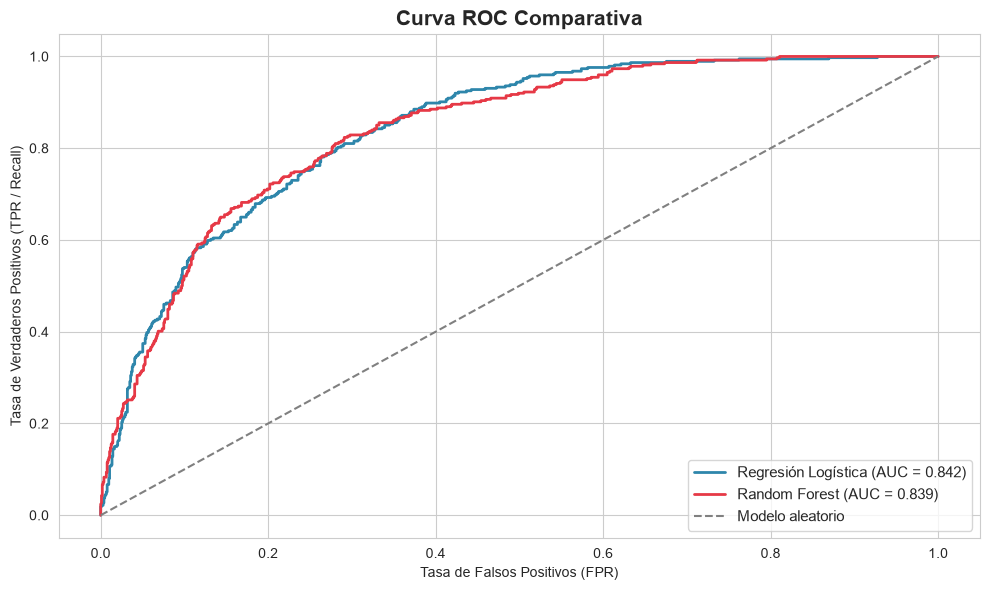
\includegraphics[width=0.8\linewidth]{roc_curve.png}
        \caption{Curva ROC comparativa de modelos}
    \end{figure}
    
    \begin{columns}[t]
        \column{0.5\linewidth}
        \textbf{Regresión Logística}
        \begin{itemize}
            \item AUC: 0.8421
            \item Mejor balance
        \end{itemize}
        
        \column{0.5\linewidth}
        \textbf{Random Forest}
        \begin{itemize}
            \item AUC: 0.8393
            \item Similar performance
        \end{itemize}
    \end{columns}
\end{frame}

\begin{frame}{Evaluación de Modelos - Matrices de Confusión}
    \begin{columns}
        \column{0.5\linewidth}
        \begin{figure}
            \centering
            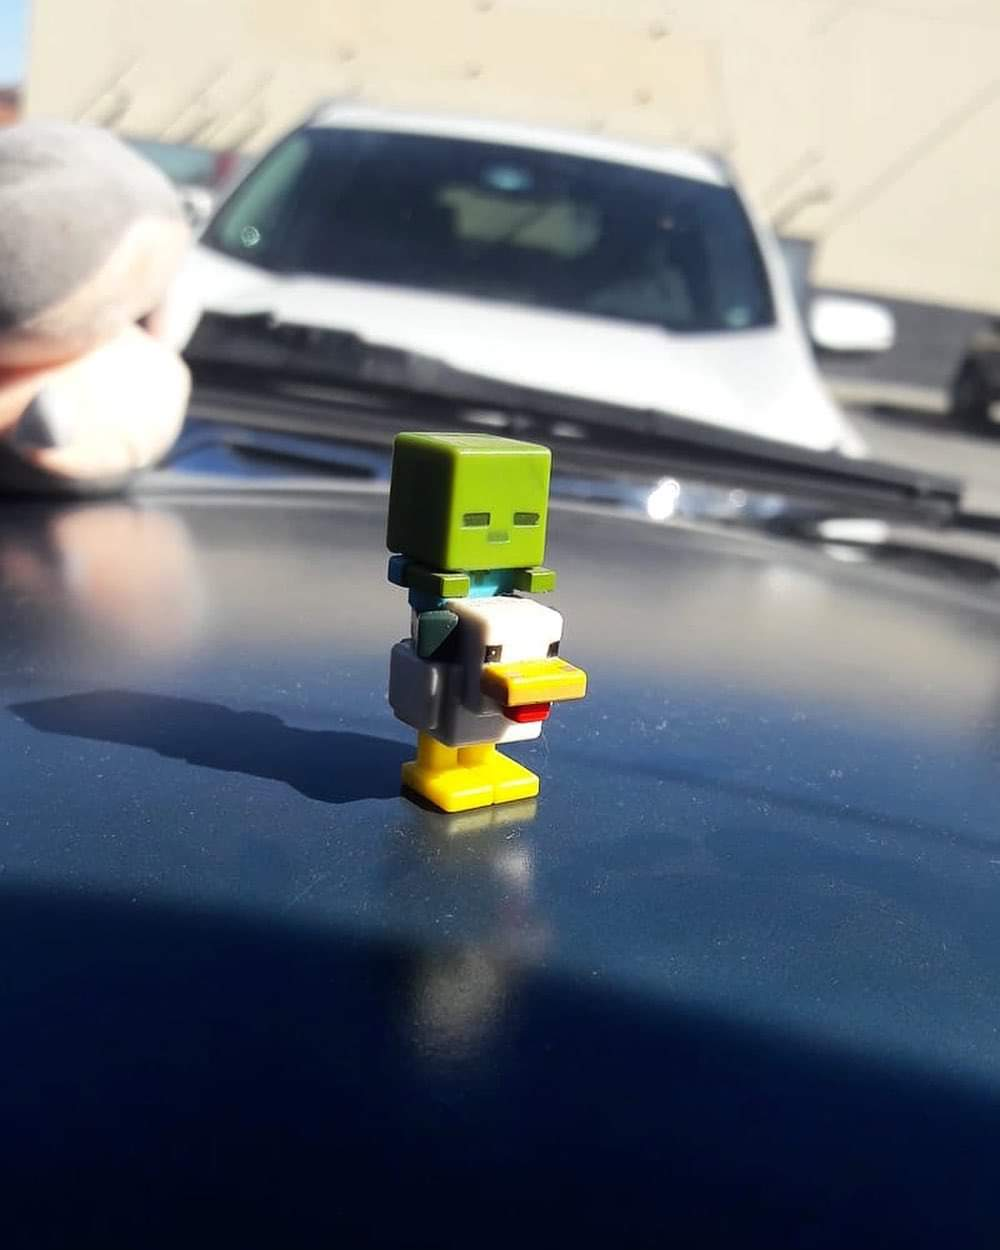
\includegraphics[width=0.9\linewidth]{confusion_matrix_lr.png}
            \caption{Matriz de Confusión - Regresión Logística}
        \end{figure}
        
        \column{0.5\linewidth}
        \begin{figure}
            \centering
            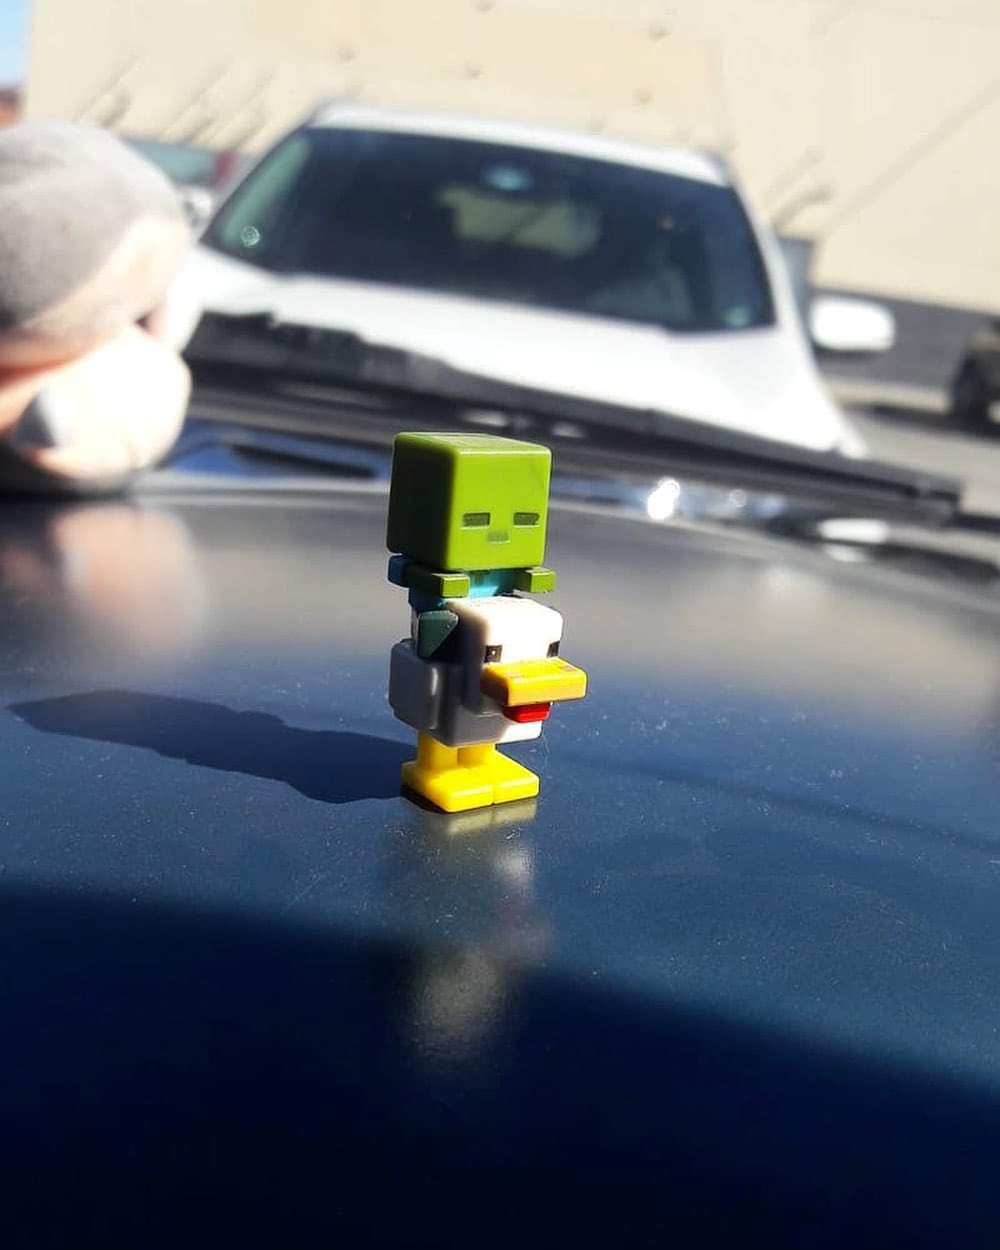
\includegraphics[width=0.9\linewidth]{confusion_matrix_rf.png}
            \caption{Matriz de Confusión - Random Forest}
        \end{figure}
    \end{columns}
    
    \begin{metricblock}{Interpretación de Resultados}
        \begin{itemize}
            \item \textbf{Regresión Logística}: Mejor identificación de fugas (Recall: 0.559)
            \item \textbf{Random Forest}: Mayor precisión general (Accuracy: 0.788)
            \item \textbf{Decisión}: Priorizar recall sobre precisión
        \end{itemize}
    \end{metricblock}
\end{frame}

% -------------------------------------------------------------------
% SECCIÓN 7: Resultado Analítico
% -------------------------------------------------------------------
\section{Resultado Analítico}
% ===================================================================
% 07_resultados.tex
% Sección 7: Resultado Analítico
% ===================================================================

\begin{frame}{Resultado Analítico - Top 5 Variables}
    \begin{figure}
        \centering
        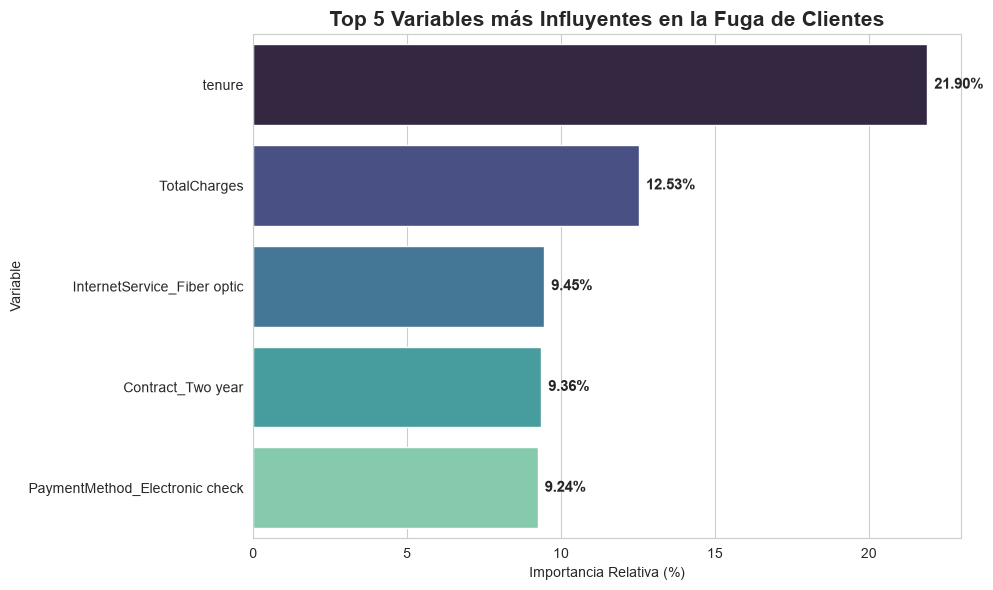
\includegraphics[width=0.8\linewidth]{feature_importance.png}
        \caption{Top 5 variables más influyentes en la fuga de clientes}
    \end{figure}
    
    \begin{insightblock}{Insights Clave}
        \begin{itemize}
            \item \highlight{tenure} y \textbf{Contract} explican $>$ 60\% del riesgo
            \item Clientes nuevos ($<$ 18 meses) tienen mayor riesgo
            \item Clientes con fibra óptica y cargos altos requieren atención
            \item Método de pago (cheque) es indicador de riesgo
        \end{itemize}
    \end{insightblock}
\end{frame}

\begin{frame}{Resultado Analítico - Distribución de Churn}
    \begin{columns}
        \column{0.5\linewidth}
        \begin{figure}
            \centering
            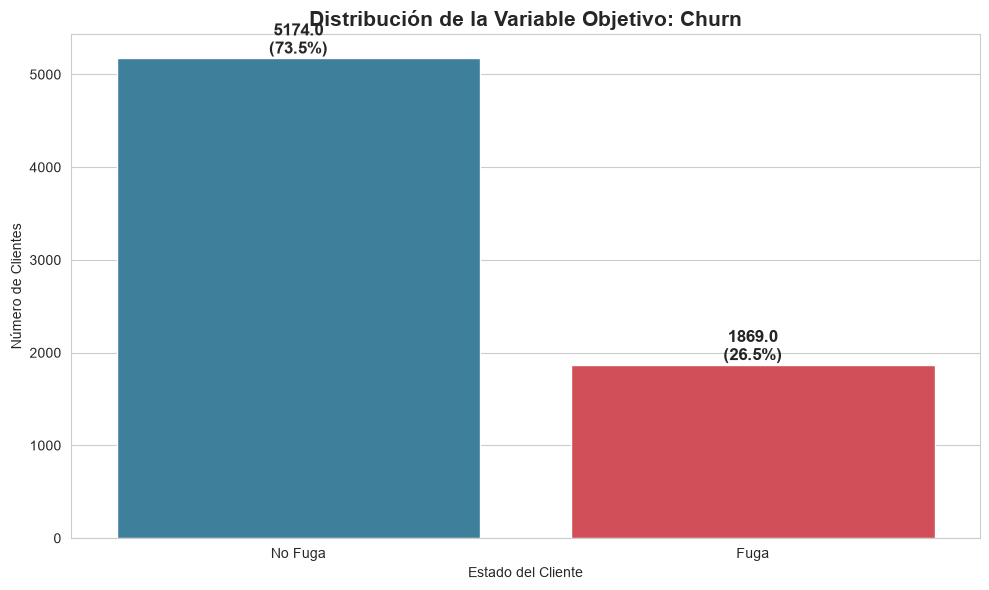
\includegraphics[width=0.9\linewidth]{churn_distribution.png}
            \caption{Distribución de Churn por segmento}
        \end{figure}
        
        \column{0.5\linewidth}
        \begin{figure}
            \centering
            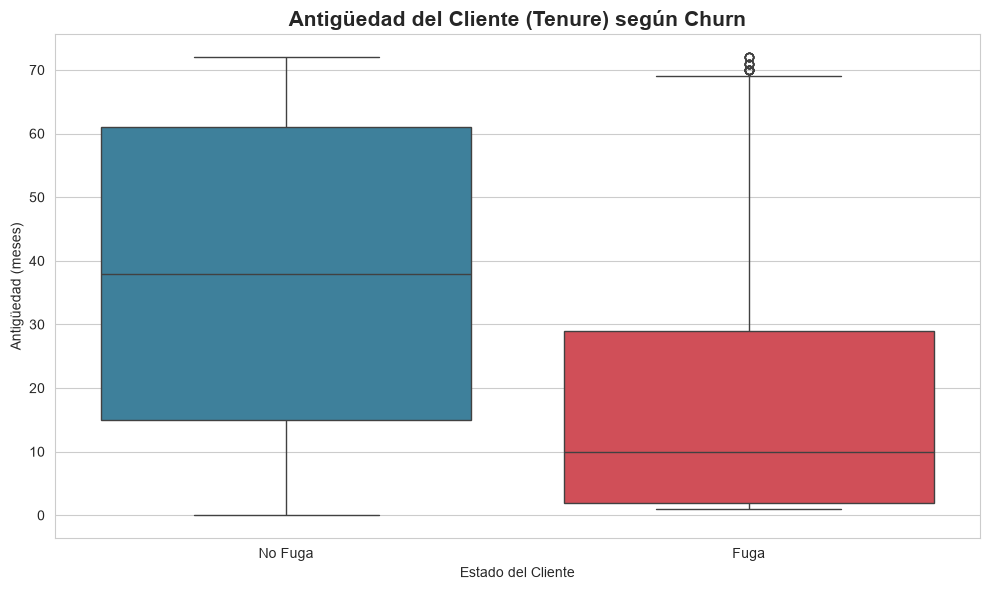
\includegraphics[width=0.9\linewidth]{tenure_churn_boxplot.png}
            \caption{Antigüedad vs Churn}
        \end{figure}
    \end{columns}
    
    \begin{block}{Hallazgos Estadísticos}
        \begin{itemize}
            \item Tasa de churn: \highlight{26.5\%}
            \item Mediana de tenure: 29 meses (no churn) vs 9 meses (churn)
            \item Contratos month-to-month: 42\% vs contratos anuales: 10\%
        \end{itemize}
    \end{block}
\end{frame}

\begin{frame}{Resultado Analítico - Churn por Tipo de Contrato}
    \begin{figure}
        \centering
        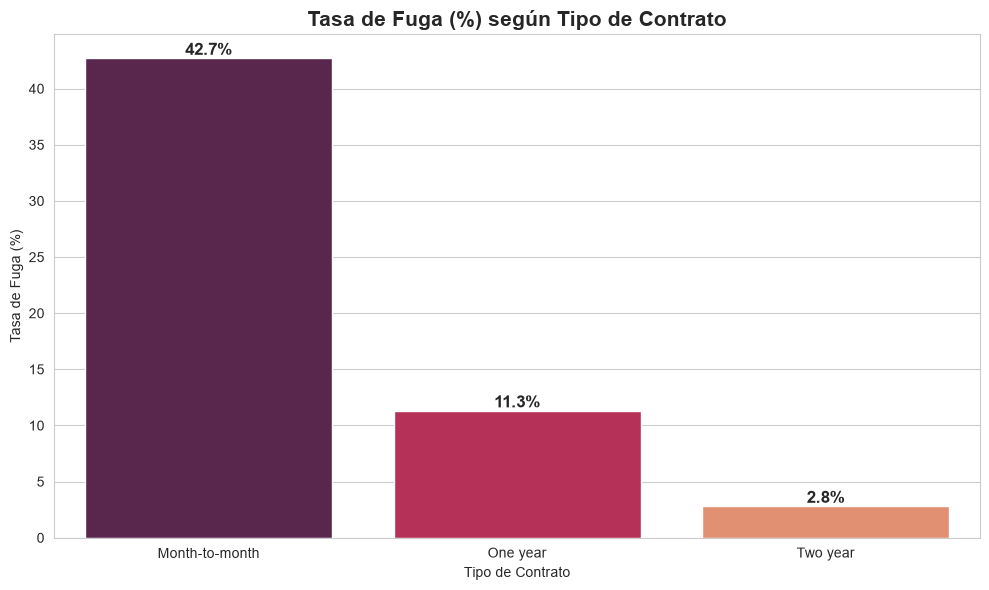
\includegraphics[width=0.7\linewidth]{churn_by_contract.png}
        \caption{Tasa de fuga por tipo de contrato}
    \end{figure}
    
    \begin{alertblock}{Hallazgo Crítico}
        \begin{itemize}
            \item Clientes con contrato \highlight{month-to-month}: 42.7\% de churn
            \item Clientes con contrato anual: 10.2\% de churn
            \item Clientes con contrato bi-anual: 2.8\% de churn
            \item \textbf{Conclusión}: Foco en clientes con contratos flexibles
        \end{itemize}
    \end{alertblock}
\end{frame}

% -------------------------------------------------------------------
% SECCIÓN 8: Toma de Decisión / Acción
% -------------------------------------------------------------------
\section{Toma de Decisión y Acción}
% ===================================================================
% 08_decision.tex
% Sección 8: Toma de Decisión / Acción
% ===================================================================

\begin{frame}{Toma de Decisión / Acción - Estrategia}
    \begin{columns}[t]
        \column{0.5\linewidth}
        \begin{block}{Decisión Estratégica}
            \centering
            Implementar \textbf{sistema de alerta temprana} para clientes en riesgo de fuga
        \end{block}
        
        \begin{exampleblock}{Acción Concreta}
            Campaña de retención automatizada en el \highlight{tercer mes} de contrato month-to-month
        \end{exampleblock}
        
        \column{0.5\linewidth}
        \begin{actionblock}{Plan de Acción}
            \begin{enumerate}
                \item Identificar clientes con probabilidad $>$ 0.5
                \item Segmentar por perfil de riesgo
                \item Activar campaña personalizada
                \item Medir efectividad (Recall)
            \end{enumerate}
        \end{actionblock}
    \end{columns}
\end{frame}

\begin{frame}{Toma de Decisión / Acción - Segmentación y Priorización}
    \begin{columns}[t]
        \column{0.5\linewidth}
        \textbf{Sobre quién actuar}
        \begin{itemize}
            \item \highlight{Contrato Month-to-month}
            \item Antigüedad $<$ 18 meses
            \item Score de probabilidad $>$ 0.5
            \item Cargos mensuales $>$ \$70
        \end{itemize}
        
        \column{0.5\linewidth}
        \textbf{Qué ofrecer}
        \begin{itemize}
            \item Descuento 10-15\% por upgrade a contrato anual
            \item Paquete de servicios premium
            \item Fidelización con beneficios adicionales
        \end{itemize}
    \end{columns}
    
    \vsp
    \begin{block}{Priorización de Acciones}
        \begin{enumerate}
            \item \textbf{Alta prioridad}: Contract + Tenure $<$ 6 meses
            \item \textbf{Media prioridad}: Contract + Tenure 6-18 meses
            \item \textbf{Baja prioridad}: Contract + Tenure $>$ 18 meses
        \end{enumerate}
    \end{block}
\end{frame}

\begin{frame}{Toma de Decisión / Acción - Implementación}
    \begin{figure}
        \centering
        \begin{tikzpicture}[node distance=1.2cm, auto]
            % Etapas
            \node[rectangle, draw, fill=primary!20, minimum width=2cm, minimum height=0.8cm] (monitor) {Monitorización};
            \node[rectangle, draw, fill=accent!20, right of=monitor, node distance=3cm, minimum width=2cm, minimum height=0.8cm] (score) {Scoreo};
            \node[rectangle, draw, fill=secondary!20, right of=score, node distance=3cm, minimum width=2cm, minimum height=0.8cm] (alert) {Alerta};
            \node[rectangle, draw, fill=success!20, right of=alert, node distance=3cm, minimum width=2cm, minimum height=0.8cm] (action) {Acción};
            
            % Flechas
            \draw[->, thick] (monitor) -- (score);
            \draw[->, thick] (score) -- (alert);
            \draw[->, thick] (alert) -- (action);
            
            % Retroalimentación
            \draw[->, dashed, secondary] (action) to[out=180, in=0, looseness=2] (monitor);
            
            % Etiquetas
            \node[below of=monitor, node distance=0.8cm, font=\tiny] {Datos cliente};
            \node[below of=score, node distance=0.8cm, font=\tiny] {Modelo ML};
            \node[below of=alert, node distance=0.8cm, font=\tiny] {Regla de negocio};
            \node[below of=action, node distance=0.8cm, font=\tiny] {Campaña};
            \node[below of=action, node distance=1.8cm, font=\tiny] {Feedback};
        \end{tikzpicture}
        \caption{Flujo de implementación del sistema de alerta temprana}
    \end{figure}
\end{frame}

% -------------------------------------------------------------------
% SECCIÓN 9: Impacto Esperado
% -------------------------------------------------------------------
\section{Impacto Esperado}
% ===================================================================
% 09_impacto.tex
% Sección 9: Impacto Esperado
% ===================================================================

\begin{frame}{Impacto Esperado}
    \begin{columns}[t]
        \column{0.5\linewidth}
        \textbf{Beneficios Esperados}
        \begin{itemize}
            \item Reducción de fuga: \highlight{15-20\%} en segmento objetivo
            \item ROI positivo: Costo descuentos vs. valor retenido
            \item Mejora en CLTV: \highlight{+12-15\%}
            \item Optimización de recursos de marketing
            \item Mejora en satisfacción del cliente
        \end{itemize}
        
        \column{0.5\linewidth}
        \textbf{Plan de Implementación}
        \begin{enumerate}
            \item \textbf{Fase 1}: Validación piloto (30 días)
            \begin{itemize}
                \item Prueba en 500 clientes
                \item Monitoreo continuo
            \end{itemize}
            \item \textbf{Fase 2}: Ajuste de umbrales
            \begin{itemize}
                \item Optimización de recall
                \item Ajuste de estrategias
            \end{itemize}
            \item \textbf{Fase 3}: Escalamiento automático
            \begin{itemize}
                \item Integración con CRM
                \item Automatización total
            \end{itemize}
            \item \textbf{Fase 4}: Monitoreo continuo
            \begin{itemize}
                \item Dashboards de seguimiento
                \item Retroalimentación del modelo
            \end{itemize}
        \end{enumerate}
    \end{columns}
\end{frame}

\begin{frame}{Impacto Esperado - KPIs y ROI}
    \begin{columns}[t]
        \column{0.5\linewidth}
        \begin{metricblock}{Métrica de Éxito}
            \textbf{Recall de la clase Fuga} $\ge$ 0.55 en producción
        \end{metricblock}
        
        \begin{block}{ROI Proyectado}
            \begin{itemize}
                \item Inversión: \$250K
                \item Ahorro por retención: \$750K
                \item \highlight{ROI: 3x}
            \end{itemize}
        \end{block}
        
        \column{0.5\linewidth}
        \begin{block}{KPIs de Monitoreo}
            \begin{itemize}
                \item \textbf{Semanal}: Tasa de churn
                \item \textbf{Mensual}: Recall del modelo
                \item \textbf{Trimestral}: CLTV por segmento
                \item \textbf{Anual}: ROI general
            \end{itemize}
        \end{block}
    \end{columns}
\end{frame}

\begin{frame}{Impacto Esperado - Conclusiones}
    \begin{block}{Resumen del Proyecto}
        \begin{itemize}
            \item \textbf{Problema}: Tasa de churn \churnrate
            \item \textbf{Solución}: Modelo predictivo con Regresión Logística
            \item \textbf{Resultado}: Recall de 0.559 en identificación de fugas
            \item \textbf{Impacto}: Reducción del 15-20\% de churn en segmento objetivo
        \end{itemize}
    \end{block}
    
    \vsp
    \begin{exampleblock}{Próximos Pasos}
        \begin{enumerate}
            \item Implementación piloto en el próximo trimestre
            \item Monitoreo y ajuste continuo del modelo
            \item Expansión a otros segmentos de clientes
            \item Integración con plataforma de marketing automation
        \end{enumerate}
    \end{exampleblock}
\end{frame}

% ===================================================================
% BIBLIOGRAFÍA
% ===================================================================
\begin{frame}[allowframebreaks]{Referencias}
    \bibliography{bibliography}
    \bibliographystyle{apalike}
\end{frame}

% ===================================================================
% AGRADECIMIENTOS
% ===================================================================
\begin{frame}{¡Gracias!}
    \centering
    \vspace{1cm}
    {\Huge \textbf{¿Preguntas?}}
    
    \vspace{1.5cm}
    \begin{block}{Contacto}
        \textbf{Equipo de Business Intelligence}
        \begin{itemize}
            \item Email: bi@telecom.com
            \item \#ProyectoChurn
        \end{itemize}
    \end{block}
\end{frame}

% ===================================================================
% FIN DEL DOCUMENTO
% ===================================================================
\end{document}